
%-----------------------------------------------------------------------------%
\chapter{\babSatu}
%-----------------------------------------------------------------------------%
Bab ini menjelaskan latar belakang, permasalahan, tujuan dan ruang lingkup 
penelitian, serta sistematika penulisan tugas akhir penelitian 

%-----------------------------------------------------------------------------%
\section{Latar Belakang}
%-----------------------------------------------------------------------------%
Seiring berjalannya waktu, teknologi informasi (IT) mengalami perkembangan yang
pesat. Optimisasi perangkat keras untuk komputasi dan kemudahan mengakses merup
akan tujuan yang ingin dicapai. Pemanfaatannya pun beragam dari media hiburan multimedia, membantu dalam
pekerjaan sehari hari, berkomunikasi dengan orang lain, dan untuk bermain \textit{video game}.
Teknologi informasi sudah lama digunakan dalam penelitian, khususnya eksperimen secara virtual. Eksperimen ini memanfaatkan kemampuan komputer dalam komputasi dan menyimpan data dalam skala besar. Teknologi informasi yang memenuhi kriteria tersebut adalah \textit{supercomputer}.Namun, hal ini tidak terlepas dari kendala yang ada.Kemampuan komputasi yang tinggi (\textit{supercomputer}) menyebabkan besarnya biaya yang harus dikeluarkan dalam pengadaan \textit{supercomputer}.
Peneliti perlu meluangkan biaya diluar biaya penelitian tersebut.Selain itu, 
peneliti juga perlu memahami hal teknis terkait dengan pengoperasian \textit{supercomputer} dan juga perawatannya. Oleh karena itu, pemanfaatan abstraksi \textit{supercomputer} dalam sebuah komputer dapat mengurangi kendala biaya yang akan dihadapi oleh peneliti. \textit{Cloud computing} juga dapat mengurangi kendala alokasi tempat \textit{supercomputer}.
\begin{figure}
	\centering
	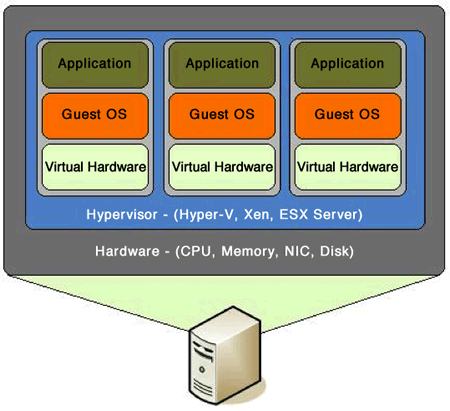
\includegraphics[scale = 0.5]{virtual_machine.png}
	\caption{\textit{virtual machine}}
	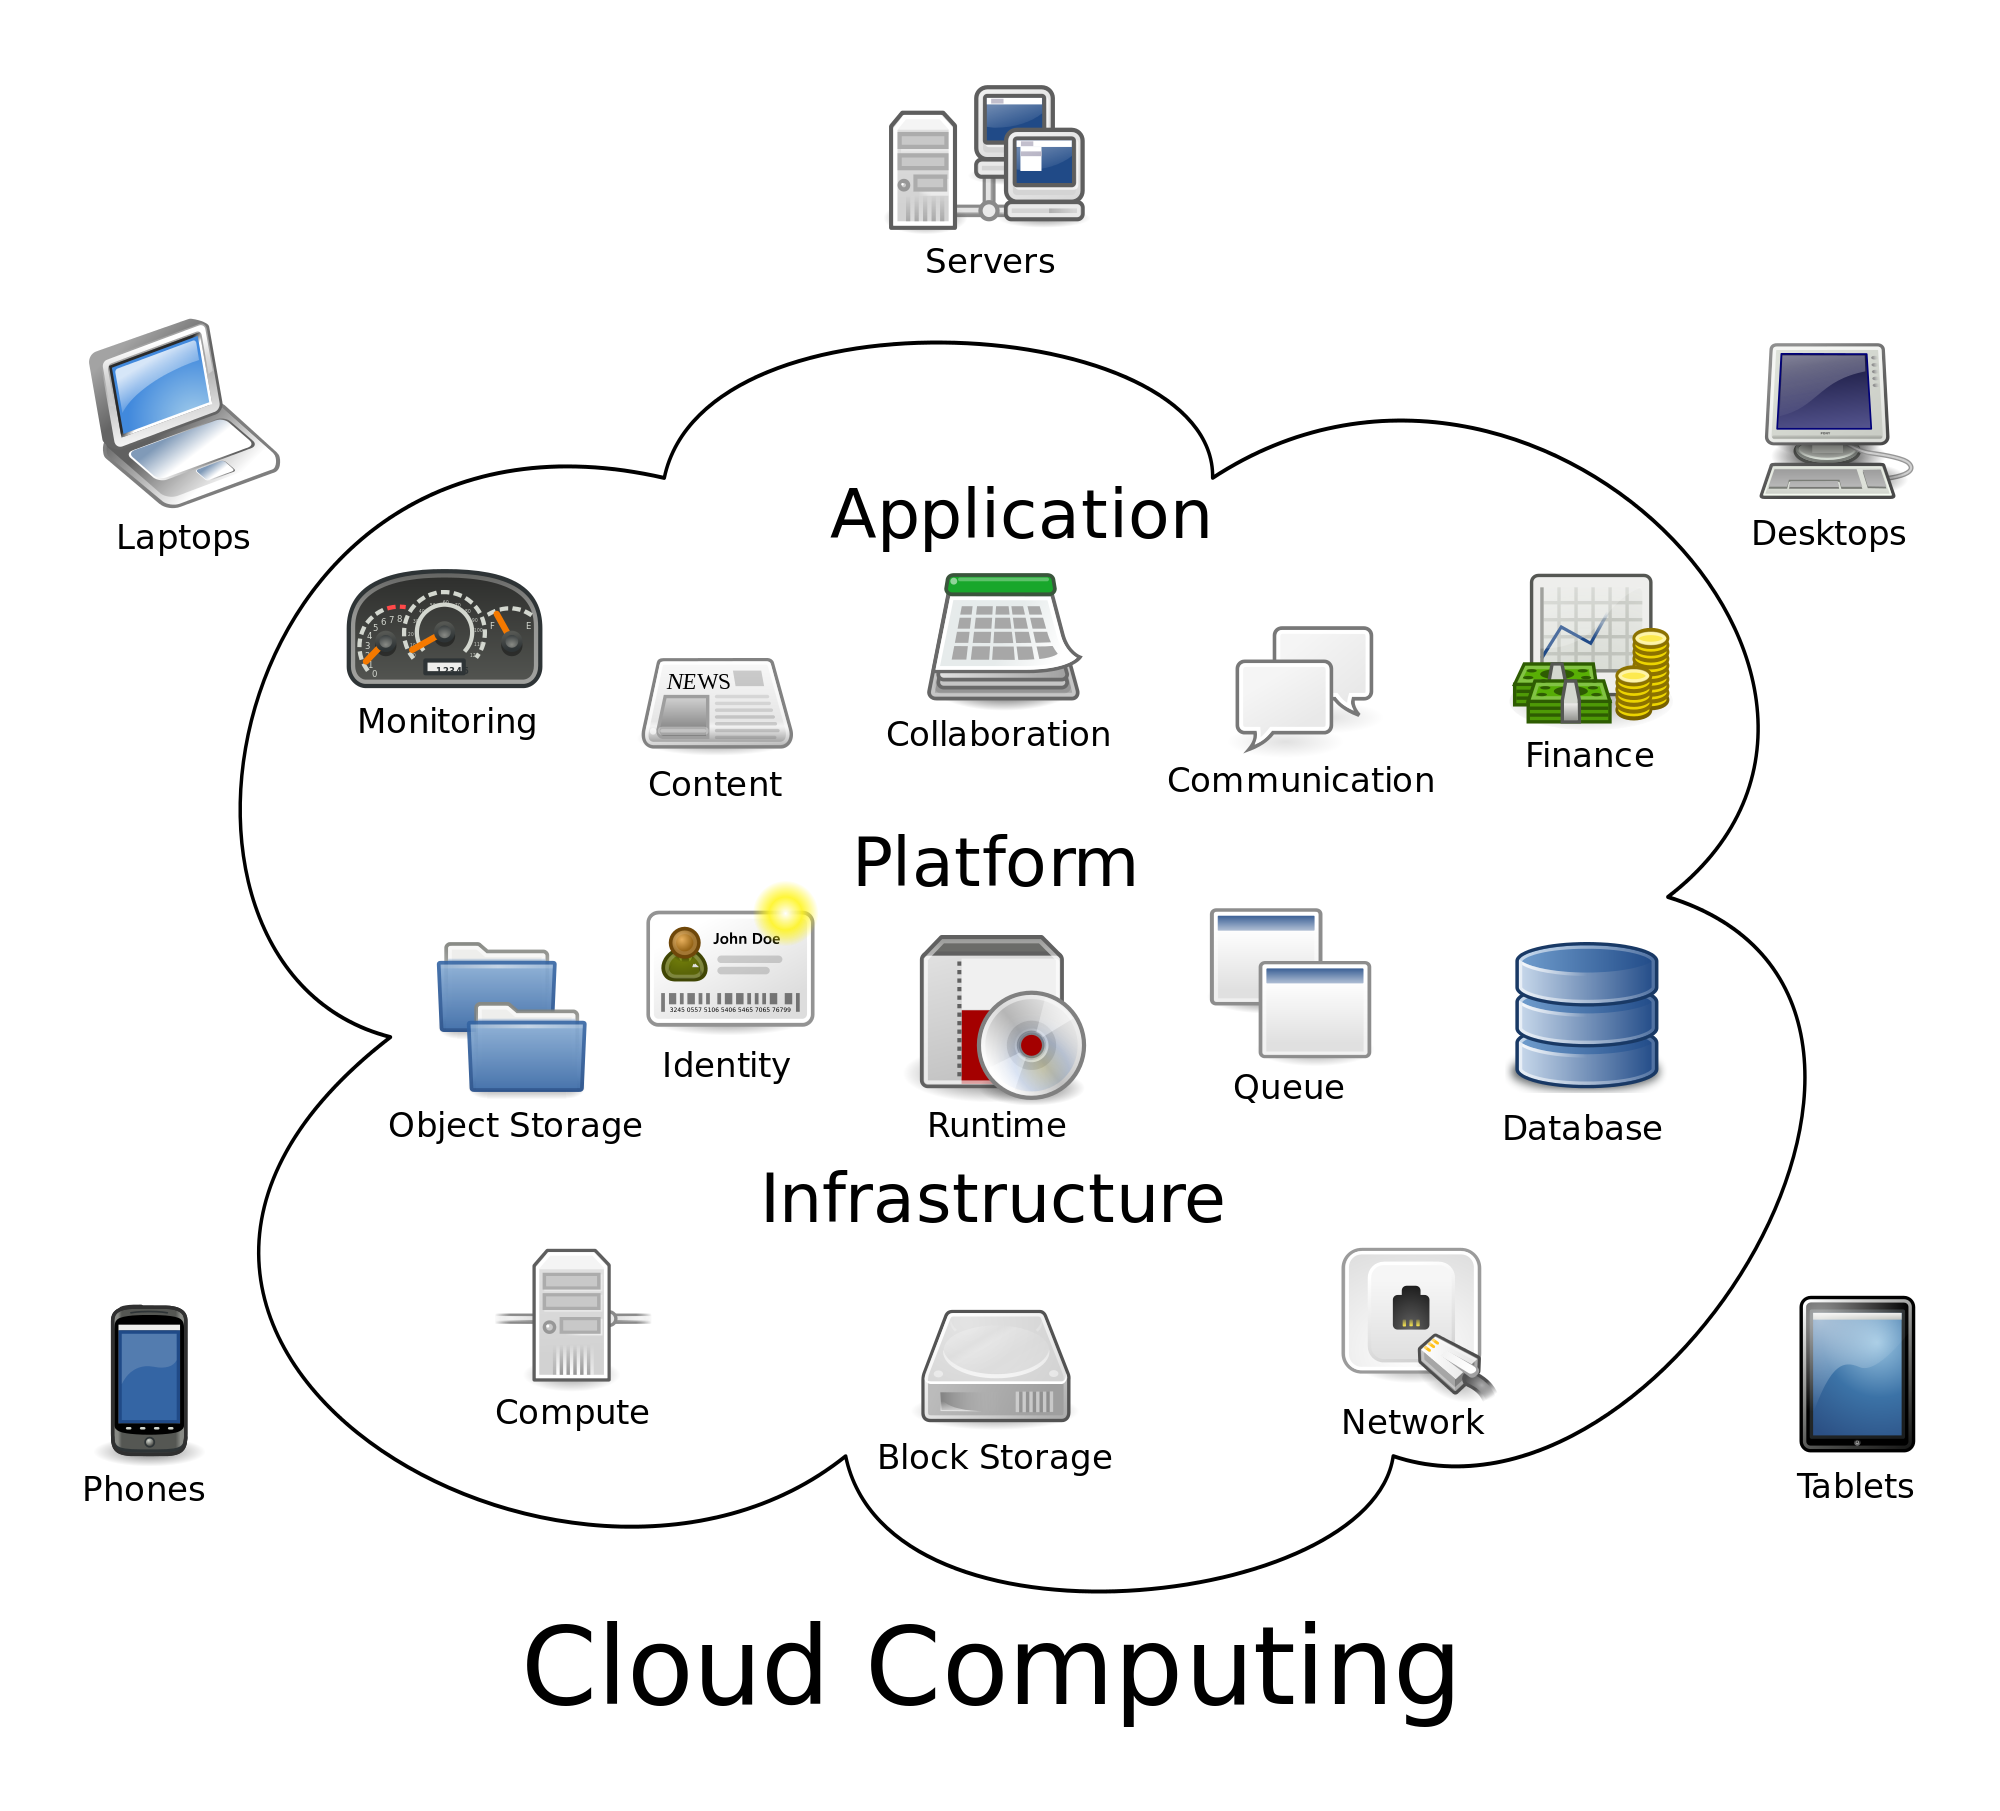
\includegraphics[scale = 0.1]{cloud_computing.png}
	\caption{\textit{cloud computing}}
\end{figure}
Salah satu bidang penelitian terkini yang menggunakan teknologi informasi dengan komputasi
tinggi adalah \textit{drug discovery}. Teknik terkait yang digunakan adalah 
\textit{virtual screening}, baik itu secara \textit{ligand-based} atau \textit{structured-based}
. Pemanfaatan teknologi \textit{cloud computing} diharapkan dapat memberikan kemudahan
bagi para peneliti tanpa perlu mempelajari secara detail pengoperasian dan perawatan teknologi yang mereka gunakan secara mendalam dan mengurangi kendala biaya dalam pengadaan \textit{supercomputer}. Dengan adanya \textit{cloud computing} peneliti juga dapat saling berbagi
\textit{resource}.

%-----------------------------------------------------------------------------%
\section{Permasalahan}
%-----------------------------------------------------------------------------%
%-----------------------------------------------------------------------------%
\subsection{Definisi Permasalahan}
%-----------------------------------------------------------------------------%
Berdasarkan latar belakang yang telah dijelaskan, penulis berusaha untuk menganalisis
apakah pemanfaatan Docker sebagai salah satu aplikasi abstraksi komputer secara \textit{virtual} dapat diajukan sebagai solusi alternatif
yang dapat digunakan dalam penelitian, khususnya terkait \textit{drug discovery}. 
Pengadaan \textit{supercomputer} secara fisik tentunya akan memakan alokasi tempat maupun biaya dalam penelitian.
Selain itu, dengan adanya \textit{cloud computing}, peneliti tidak dituntut untuk memahami
teknologi terkait secara mendalam, cukup fokus dengan penelitian yang sedang dikerjakan. Peneliti juga dapat dengan mudah saling berbagi \textit{resource}, baik itu sumber komputasi maupun data mentah maupun yang telah diolah.  
Aplikasi yang digunakan dalam tugas akhir ini adalah Autodock dan Autodock Vina bertugas untuk \textit{virtual screening}.


%-----------------------------------------------------------------------------%
\subsection{Batasan Permasalahan}
%-----------------------------------------------------------------------------%
Pada penelitian ini, penulis tidak akan berfokus pada \textit{virtual screening} yang akan dilakukan.Penulis mencoba untuk menganalasis apakah kinerja Docker setara atau lebih baik dibandingkan dengan \textit{cluster} dan 
\textit{grid computing} dalam melakukan \textit{drug discovery}. 


%-----------------------------------------------------------------------------%
\section{Tujuan}
%-----------------------------------------------------------------------------%
Penelitian ini secara umum bertujuan untuk mengenalkan pemanfaatan abstraksi komputer secara \textit{virtual} dibantu dengan teknologi \textit{cloud computing}
sebagai alternatif pengadaan \textit{supercomputer} secara fisik terkait dengan penelitian dengan menggunakan komputasi yang tinggi, khususnya \textit{drug discovery}
dalam bidang farmakologi. Selain itu, Penelitian ini secara khusus untuk menganalisis kinerja Docker
dalam menjalankan Autodock maupun Autodock Vina.


%-----------------------------------------------------------------------------%
\section{Posisi Penelitian}
%-----------------------------------------------------------------------------%
Penelitian ini merupakan lanjutan dari topik yang sedang dilakukan oleh Bapak Muhammad Hafizhuddin Hilman, S.Kom., M.Kom. 

%-----------------------------------------------------------------------------%
\section{Sistematika Penulisan}
%-----------------------------------------------------------------------------%
Penulisan ini terbagi dalam 5 bab :
\begin{itemize}
	\item BAB 1 \babSatu \\
	Bagian ini berisikan latar belakang, permasalahan, tujuan dan ruang lingkup penelitian, serta sistematika penulisan tugas akhir penelitian. 
	\item BAB 2 \babDua \\
	Bagian ini berisikan penjelasan \textit{drug discovery} dengan cara \textit{virtual screening} memanfaatkan teknologi informasi secara umum. Selain itu, \textit{cloud computing} dan Docker akan dijelaskan secara detail.
	\item BAB 3 \babTiga \\
	Bagian ini berisikan detail tahap-tahap penelitian dan data yang digunakan.
	\item BAB 4 \babEmpat \\
	Bagian ini berisikan hasil dari penelitian yang telah dilaksanakan dan analisis dari hasil yang diperoleh.
	\item BAB 5 \kesimpulan \\
	Bagian ini berisikan kesimpulan penulis terkait dengan penelitian dan saran penulis dalam penelitian ke depannya.
\end{itemize}


